\documentclass[tikz]{standalone}
\usepackage[utf8]{inputenc}
\usetikzlibrary{calc}

\definecolor{mycolor}{RGB}{12,18,33}

\newcommand{\AK}{\texttt{AK}}
\newcommand{\SB}{\texttt{SB}}
\newcommand{\MC}{\texttt{MC}}
\newcommand{\SR}{\texttt{SR}}

\newcommand{\aesbox}[2]{\draw[line width=1.5pt] (#1,#2) rectangle ($(#1,#2) + (1,1)$);}

\begin{document}
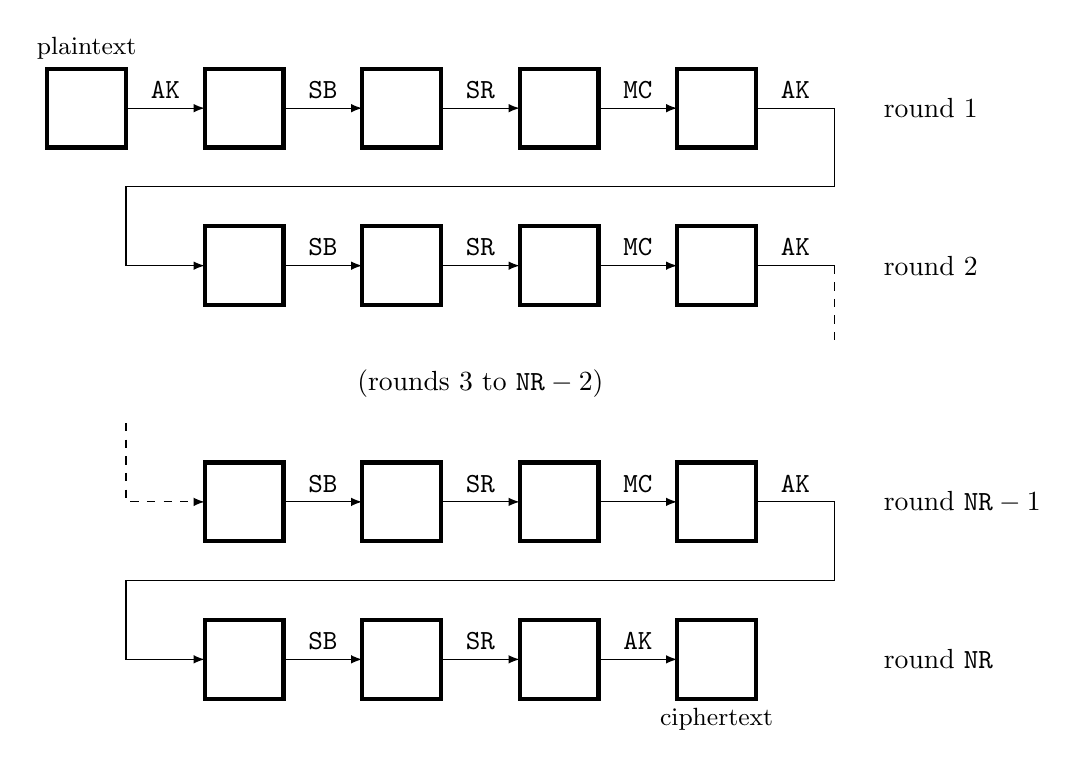
\begin{tikzpicture}
% round NR
\aesbox{0}{0}
\aesbox{2}{0}
\aesbox{4}{0}
\aesbox{6}{0}

% round NR - 1
\aesbox{0}{2}
\aesbox{2}{2}
\aesbox{4}{2}
\aesbox{6}{2}

% round 2
\aesbox{0}{5}
\aesbox{2}{5}
\aesbox{4}{5}
\aesbox{6}{5}

% round 1
\aesbox{0}{7}
\aesbox{2}{7}
\aesbox{4}{7}
\aesbox{6}{7}
\aesbox{-2}{7}

% arrows
\draw[-latex] (-1, 7.5) --++ (1, 0) node[above,midway] {\AK};

\draw[-latex] (1, 7.5) --++ (1, 0) node[above,midway] {\SB};
\draw[-latex] (3, 7.5) --++ (1, 0) node[above,midway] {\SR};
\draw[-latex] (5, 7.5) --++ (1, 0) node[above,midway] {\MC};
\draw[-latex] (7, 7.5) --++ (1, 0) node[above,midway] {\AK} --++ (0,-1) --++ (-9,0) --++ (0,-1) --++ (1,0);

\draw[-latex] (1, 5.5) --++ (1, 0) node[above,midway] {\SB};
\draw[-latex] (3, 5.5) --++ (1, 0) node[above,midway] {\SR} ;
\draw[-latex] (5, 5.5) --++ (1, 0) node[above,midway] {\MC};
\draw (7, 5.5) --++ (1, 0) node[above,midway] {\AK};
\draw[dashed] (8,5.5) --++ (0, -1);

\draw[dashed,-latex] (-1, 3.5) -- (-1, 2.5) -- (0,2.5);
\draw[-latex] (1, 2.5) --++ (1, 0) node[above,midway] {\SB};
\draw[-latex] (3, 2.5) --++ (1, 0) node[above,midway] {\SR} ;
\draw[-latex] (5, 2.5) --++ (1, 0) node[above,midway] {\MC};
\draw[-latex] (7, 2.5) --++ (1, 0) node[above,midway] {\AK} --++ (0,-1) --++ (-9,0) --++ (0,-1) --++ (1,0);

\draw[-latex] (1, .5) --++ (1, 0) node[above,midway] {\SB};
\draw[-latex] (3, .5) --++ (1, 0) node[above,midway] {\SR};
\draw[-latex] (5, .5) --++ (1, 0) node[above,midway] {\AK};

% text
\node[right] at (8.5, 7.5) {round $1$};
\node[right] at (8.5, 5.5) {round $2$};
\node at (3.5, 4) {(rounds $3$ to $\texttt{NR} - 2$)};
\node[right] at (8.5, 2.5) {round $\texttt{NR} - 1$};
\node[right] at (8.5, .5) {round $\texttt{NR}$};

\node[above] at (-1.5, 8) {\small plaintext};
\node[below] at (6.5, 0) {\small ciphertext};
\end{tikzpicture}
\end{document}